% ---------------------------------------------------------------------------
%  Shared code across repositories: the drwho scheme
%  Harrison B. Prosper
% ---------------------------------------------------------------------------
\documentclass[11pt,a4paper]{article}

\usepackage[T1]{fontenc}
\usepackage[utf8]{inputenc}
\usepackage{charter}
\usepackage[scaled=0.92]{helvet}
\usepackage{courier}
\usepackage{amsmath}
\usepackage{microtype}
\usepackage[margin=2.4cm,top=2.6cm,bottom=2.6cm]{geometry}
\usepackage{xcolor}
\usepackage{listings}
\usepackage{array}
\usepackage{booktabs}
\usepackage{enumitem}
\usepackage{titlesec}
\usepackage{tcolorbox}
\usepackage{tikz}
\usepackage{fancyhdr}
\usepackage{caption}
\usepackage{needspace}
\usepackage[hidelinks]{hyperref}

\tcbuselibrary{skins,breakable}
\usetikzlibrary{arrows.meta,positioning,shapes.geometric}

% ------------------------------------------------ colours
\definecolor{ink}{HTML}{1A1A1A}
\definecolor{accent}{HTML}{1F4E79}
\definecolor{accentlight}{HTML}{E8EFF6}
\definecolor{rule}{HTML}{8C3B12}
\definecolor{rulelight}{HTML}{FBEDE6}
\definecolor{codebg}{HTML}{F6F7F8}
\definecolor{codeframe}{HTML}{D8DCE0}
\definecolor{comment}{HTML}{4E7A4E}
\definecolor{keyword}{HTML}{1F4E79}
\definecolor{strng}{HTML}{8C3B12}

\color{ink}

% ------------------------------------------------ headings
\titleformat{\section}{\sffamily\large\bfseries\color{accent}}{\thesection}{0.7em}{}
\titleformat{\subsection}{\sffamily\normalsize\bfseries\color{accent}}{\thesubsection}{0.6em}{}
\titlespacing*{\section}{0pt}{1.6em plus .3em}{0.7em}
\titlespacing*{\subsection}{0pt}{1.2em plus .2em}{0.5em}

\pagestyle{fancy}
\fancyhf{}
\renewcommand{\headrulewidth}{0.3pt}
\fancyhead[L]{\sffamily\footnotesize\color{accent}Shared code across repositories}
\fancyhead[R]{\sffamily\footnotesize\color{accent}\thepage}

% ------------------------------------------------ listings
\lstdefinestyle{base}{
  basicstyle=\ttfamily\footnotesize,
  backgroundcolor=\color{codebg},
  frame=single,
  rulecolor=\color{codeframe},
  framesep=5pt,
  xleftmargin=6pt,
  xrightmargin=2pt,
  breaklines=true,
  breakatwhitespace=false,
  postbreak=\mbox{\textcolor{codeframe}{$\hookrightarrow$}\space},
  showstringspaces=false,
  columns=fullflexible,
  keepspaces=true,
  aboveskip=0.9em,
  belowskip=0.9em,
  commentstyle=\color{comment}\itshape,
  keywordstyle=\color{keyword}\bfseries,
  stringstyle=\color{strng},
}
\lstdefinelanguage{toml}{
  morekeywords={},
  morecomment=[l]{\#},
  morestring=[b]",
  moredelim=[s][\color{keyword}\bfseries]{[}{]},
}
\lstset{style=base}
\lstdefinestyle{sh}{style=base,language=bash,
  keywordstyle=\color{ink},
  morekeywords={git,pip,python,cd,conda}}
\lstdefinestyle{py}{style=base,language=Python}
\lstdefinestyle{tomlst}{style=base,language=toml}
\lstdefinestyle{plain}{style=base,language=}

% ------------------------------------------------ callout boxes
\newtcolorbox{rulebox}[1][]{
  breakable, enhanced, colback=rulelight, colframe=rule,
  boxrule=0pt, leftrule=2.5pt, arc=1pt, left=8pt, right=8pt, top=6pt, bottom=6pt,
  colbacktitle=rulelight, titlerule=0mm, toptitle=2pt, bottomtitle=0pt,
  fonttitle=\sffamily\bfseries\small, coltitle=rule, title={#1}}
\newtcolorbox{notebox}[1][]{
  breakable, enhanced, colback=accentlight, colframe=accent,
  boxrule=0pt, leftrule=2.5pt, arc=1pt, left=8pt, right=8pt, top=6pt, bottom=6pt,
  colbacktitle=accentlight, titlerule=0mm, toptitle=2pt, bottomtitle=0pt,
  fonttitle=\sffamily\bfseries\small, coltitle=accent, title={#1}}

\newcommand{\pkg}[1]{\texttt{#1}}
\setlist[itemize]{leftmargin=1.2em,itemsep=0.25em,topsep=0.4em}
\setlist[enumerate]{leftmargin=1.5em,itemsep=0.35em,topsep=0.4em}

% ---------------------------------------------------------------------------
\begin{document}

\begin{titlepage}
\centering
\vspace*{3.5cm}
{\sffamily\Huge\bfseries\color{accent} Shared Code Across Repositories\par}
\vspace{0.8cm}
{\sffamily\Large A scheme built on \texttt{drwho}, with \texttt{dihiggs} as the worked example\par}
\vspace{2.2cm}
{\large Harrison B. Prosper\par}
\vspace{0.3cm}
{\normalsize Department of Physics, Florida State University\par}
\vspace{2.5cm}
\begin{minipage}{0.8\textwidth}
\small
\begin{notebox}[Summary]
Common code that had been copied into several repositories now lives in one
package, \pkg{drwho}. Dependent repositories declare it as a \textsc{pep}~508
direct reference to its GitHub URL, so a user who clones a repository and runs
\texttt{pip install -e .} gets everything, with no extra step and nothing to
explain. This document records how that is set up, why each piece is the way it
is, and---most importantly---the protocol for shipping a fix so that it actually
reaches the people using it.
\end{notebox}
\end{minipage}
\vfill
{\small Version 1.0 \quad\textbullet\quad 22 September 2026 \quad\textbullet\quad
describes \pkg{drwho} 0.2.0\par}
\end{titlepage}

\tableofcontents
\thispagestyle{empty}
\clearpage
\setcounter{page}{1}

% ===========================================================================
\section{The problem}

Several repositories under \texttt{github.com/hbprosper} carried byte-identical
copies of the same utility modules. That duplication was deliberate: it made each
repository self-contained, so a student could clone one thing and run it without
first assembling an environment. The cost is the usual one. A fix applied in one
copy does not reach the others, the copies drift apart, and after a while nobody
can say which version is authoritative.

The goal is to remove the duplication \emph{without} removing the property that
made it attractive. A student should still clone one repository, run one command,
and have a working environment. They should not need to know that a second
repository exists.

% ===========================================================================
\section{The scheme}

One repository, \pkg{drwho}, holds the shared code. Every dependent repository
names it in the \texttt{dependencies} list of its \texttt{pyproject.toml}, not by
version but by URL:

\begin{lstlisting}[style=tomlst]
[project]
name = "dihiggs"
dependencies = [
    "drwho @ git+https://github.com/hbprosper/drwho.git@main",
    "numpy",
    "pandas",
    "matplotlib",
    "torch",
]
\end{lstlisting}

That is a \textsc{pep}~508 \emph{direct reference}. When pip installs the
dependent package it clones \pkg{drwho}, builds it, and installs it like any
other dependency. The user sees one extra line scroll past.

\begin{center}
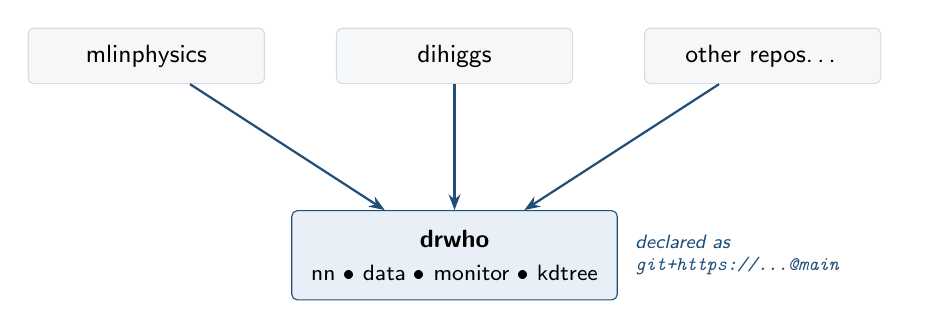
\begin{tikzpicture}[
  node distance=9mm,
  box/.style={draw=codeframe, fill=codebg, rounded corners=2pt, inner sep=6pt,
              font=\sffamily\small, minimum width=30mm, align=center},
  core/.style={draw=accent, fill=accentlight, rounded corners=2pt, inner sep=7pt,
              font=\sffamily\small\bfseries, minimum width=34mm, align=center},
  arr/.style={-{Stealth[length=2mm]}, draw=accent, thick}
]
\node[box] (a) {mlinphysics};
\node[box, right=of a] (b) {dihiggs};
\node[box, right=of b] (c) {other repos\ldots};
\node[core, below=16mm of b] (d) {drwho\\[1pt]\footnotesize\mdseries nn \textbullet\ data \textbullet\ monitor \textbullet\ kdtree};
\draw[arr] (a) -- (d);
\draw[arr] (b) -- (d);
\draw[arr] (c) -- (d);
\node[font=\sffamily\scriptsize\itshape, right=1mm of d.east, text width=32mm,
      anchor=west, color=accent]
     {declared as\\ \texttt{git+https://\ldots @main}};
\end{tikzpicture}
\end{center}

\begin{notebox}[Why not PyPI?]
Publishing to PyPI would also work, and would be slightly smoother still---no
git needed at install time, and proper version resolution. It was rejected here
because this code is not intended to be ``official''. The consequence is worth
knowing: \textsc{pep}~508 direct references are forbidden in packages uploaded to
PyPI, so adopting this scheme forecloses publishing these particular
repositories later without changing the dependency line first.
\end{notebox}

% ===========================================================================
\section{The shared repository: \texttt{drwho}}

\subsection{Layout}

\begin{lstlisting}[style=plain]
drwho/
|-- pyproject.toml
|-- README.md
|-- LICENSE
|-- .gitignore
|-- docs/
`-- drwho/
    |-- __init__.py        <- version lives here; lazy submodule loading
    |-- data.py
    |-- kdtree.py
    |-- monitor.py
    |-- nn.py
    `-- bin/
        |-- __init__.py
        `-- monitor_losses.py   <- the "monlosses" console script
\end{lstlisting}

The repository and the package share a name, which is the usual convention and
makes the path from \texttt{pip install} to \texttt{import} obvious.

\subsection{\texttt{pyproject.toml}}

\begin{lstlisting}[style=tomlst]
[build-system]
requires = ["setuptools>=77"]
build-backend = "setuptools.build_meta"

[project]
name = "drwho"
dynamic = ["version"]
description = "Shared utilities for Harrison Prosper's physics and ML course repositories"
readme = "README.md"
requires-python = ">=3.10"
license = "MIT"
license-files = ["LICENSE"]
authors = [{name = "Harrison B. Prosper", email = "hprosper@fsu.edu"}]
dependencies = [
    "numpy", "scipy", "pandas", "matplotlib",
    "torch", "requests", "pyyaml",
]

[project.optional-dependencies]
tensorboard = ["tensorboard"]

[project.urls]
Homepage = "https://github.com/hbprosper/drwho"

[tool.setuptools]
packages = ["drwho", "drwho.bin"]

[tool.setuptools.dynamic]
version = {attr = "drwho.__version__"}

[project.scripts]
monlosses = "drwho.bin.monitor_losses:main"
\end{lstlisting}

Four points deserve comment.

\paragraph{Table order matters in TOML.}
Everything written after a \texttt{[table]} header belongs to that table. A
\texttt{dependencies} list placed after \texttt{[project.urls]} silently becomes
a key \emph{inside} that table, and is never seen as a dependency list at all.
Keep every bare key of \texttt{[project]} above the first sub-table header.

\paragraph{Dependencies are unpinned, and that is deliberate.}
Colab ships a \pkg{torch} build matched to its own \textsc{cuda} driver, and so
does the university cluster. An upper bound such as
\texttt{torch>=2.4,<2.6} would, on the wrong day, make pip download several
gigabytes mid-class, possibly landing a \textsc{cpu}-only or driver-mismatched
build and demanding a runtime restart. With no bound, pip sees the requirement
already satisfied and skips it entirely.

\paragraph{\texttt{packages} is explicit.}
Left to auto-discovery with \texttt{where = ["."]}, setuptools will sweep up any
top-level directory it mistakes for a package. In \pkg{dihiggs} it had recorded
\texttt{Kurtis}, \texttt{code}, \texttt{data} and \texttt{docs} as installed
top-level names. Naming the packages explicitly avoids this, and a subpackage
such as \texttt{drwho.bin} must be listed---otherwise it is not shipped, and the
console script that points into it is dead on arrival.

\paragraph{A subpackage needs \texttt{\_\_init\_\_.py}.}
\texttt{drwho/bin/\_\_init\_\_.py} exists so that \texttt{drwho.bin} is a regular
package. Without it an editable install may still work, via the namespace-package
fallback, while a normal wheel install quietly omits the directory---a difference
that will not show up until somebody installs it the ordinary way.

\subsection{One place for the version number}

\texttt{pyproject.toml} declares \texttt{dynamic = ["version"]} and reads the
value from the package itself. The number therefore lives in exactly one place:

\begin{lstlisting}[style=py]
# drwho/__init__.py
__version__ = "0.2.0"
\end{lstlisting}

setuptools extracts this by parsing the syntax tree, so nothing is imported and
\pkg{torch} is not needed at build time. Since the version must be bumped on
\emph{every} release (Section~\ref{sec:protocol}), having two places to edit
would be a standing invitation to get them out of step.

\subsection{Lazy submodule loading}

\texttt{drwho/\_\_init\_\_.py} implements \textsc{pep}~562 module-level
\texttt{\_\_getattr\_\_}:

\begin{lstlisting}[style=py]
import importlib as _importlib

__version__ = "0.2.0"
__all__ = ["data", "kdtree", "monitor", "nn"]

def __getattr__(name):
    """Import drwho.<name> on first access (PEP 562)."""
    if name in __all__:
        return _importlib.import_module(f".{name}", __name__)
    raise AttributeError(f"module {__name__!r} has no attribute {name!r}")
\end{lstlisting}

So \texttt{import drwho} costs essentially nothing and does not drag in
\pkg{torch}; \texttt{drwho.nn} resolves on first touch. Both
\texttt{from drwho import nn} and \texttt{import drwho.nn} continue to work
unchanged.

The same principle applies inside \texttt{monitor.py}, where
\texttt{torch.utils.tensorboard} is imported by a helper rather than at module
level. An optional dependency should be probed when it is asked for, not
announced to everyone who imports the module.

% ===========================================================================
\section{A dependent repository: \texttt{dihiggs}}

\subsection{Layout after migration}

\begin{lstlisting}[style=plain]
dihiggs/
|-- pyproject.toml
|-- README.md  LICENSE  .gitignore
|-- code/              <- notebooks, run from here
|   |-- heft_prepare_data.ipynb
|   |-- heft_test.ipynb
|   |-- heft_train.ipynb
|   `-- figures/.gitkeep
|-- data/              <- tracked input data
|-- docs/
|-- clutter/           <- git-ignored; holds retired files pending deletion
`-- dihiggs/
    |-- __init__.py
    `-- heftnet.py     <- the physics: HEFTNet, FEATURES, TARGET
\end{lstlisting}

What remains in the \pkg{dihiggs} package is what is genuinely specific to
\pkg{dihiggs}. Everything generic moved to \pkg{drwho}: 1\,120 lines of
duplicated code deleted.

\subsection{Verifying that nothing is lost}

Before deleting a duplicated module, confirm that the shared copy is a superset.
Comparing file sizes is not enough; compare the \emph{interface}. Parsing both
files and comparing every top-level function and class, and every method within
each class, gave for \pkg{dihiggs}:

\begin{center}
\small
\begin{tabular}{lcccc}
\toprule
module & identical & body differs & only local & only in \pkg{drwho} \\
\midrule
\texttt{nn.py}      & 11 & 2 & \texttt{elapsed\_time} & 4 \\
\texttt{data.py}    &  3 & 0 & --- & 2 \\
\texttt{monitor.py} &  2 & 3 & --- & 2 \\
\bottomrule
\end{tabular}
\end{center}

No method existed only in the local copies. Every signature difference was an
added keyword argument with a default---\texttt{Config} gained
\texttt{dirpath} and \texttt{mkdir}, \texttt{Monitor} gained
\texttt{use\_tensorboard} and \texttt{same\_line}, \texttt{terminate} gained
\texttt{delay}---so existing call sites were unaffected. The single local-only
function, \texttt{elapsed\_time}, had moved to \texttt{drwho.monitor} and was
not called anywhere.

\begin{rulebox}[Do this before deleting anything]
Compare interfaces, not line counts. A method present only in the copy you are
about to delete is the one thing that will break, and it will break later,
in someone else's hands.
\end{rulebox}

\subsection{What changed in the notebooks}

Because the module aliases were kept identical, not one line of notebook body
code had to change. Only the import lines moved:

\begin{center}
\small
\begin{tabular}{ll}
\toprule
before & after \\
\midrule
\texttt{import dihiggs.nn as mlp}            & \texttt{import drwho.nn as mlp} \\
\texttt{import dihiggs.utils.data as dat}    & \texttt{import drwho.data as dat} \\
\texttt{import dihiggs.utils.monitor as mon} & \texttt{import drwho.monitor as mon} \\
\texttt{import heftnet as NN}                & \texttt{from dihiggs import heftnet as NN} \\
\bottomrule
\end{tabular}
\end{center}

Five lines across three notebooks. The last of these also removed a
\texttt{sys.path.insert(0, '.')} hack: once \pkg{dihiggs} is a properly installed
package, \texttt{heftnet} is reachable by import from any working directory.

\begin{notebox}[Keep the aliases]
Choosing \texttt{mlp}, \texttt{dat}, \texttt{mon} to match the old names turns a
migration into a search-and-replace on import lines. It is worth some awkwardness
in the alias names to get this.
\end{notebox}

% ===========================================================================
\section{Installing}

\subsection{Laptop or cluster}

\begin{lstlisting}[style=sh]
git clone https://github.com/hbprosper/dihiggs
cd dihiggs
pip install -e .
\end{lstlisting}

pip reads the direct reference, clones \pkg{drwho}, builds it, installs it, and
then installs \pkg{dihiggs} in editable mode. \pkg{drwho} lands non-editable in
\texttt{site-packages}, which is the right default: it is shared code, not
something a student should be editing in place.

\subsection{Colab}

Git installs work normally on Colab. Do \emph{not} clone and then
\texttt{pip install -e .}; install the whole thing from the URL in one line, and
let the direct reference pull \pkg{drwho} transitively. As the first cell of
every notebook:

\begin{lstlisting}[style=py]
import sys, subprocess
IN_COLAB = "google.colab" in sys.modules
if IN_COLAB:
    subprocess.run([sys.executable, "-m", "pip", "install", "-q",
        "dihiggs @ git+https://github.com/hbprosper/dihiggs.git@main"],
        check=True)
\end{lstlisting}

This is a no-op locally and on the cluster, where the package is already
installed. Two Colab-specific points:

\begin{itemize}
\item Every Colab runtime starts empty, so pip clones fresh each time. The stale
      version problem described in Section~\ref{sec:protocol} is a
      \emph{local}-install problem only; on Colab, \texttt{@main} always gives
      current code.
\item Keep the shared repository lean---no data files, no notebooks with stored
      outputs. It is cloned on every student's every runtime.
\end{itemize}

\subsection{Keep both repositories public}

A private repository means students pasting personal access tokens into notebook
cells: a hassle, and a bad habit to teach.

% ===========================================================================
\section{The release protocol}\label{sec:protocol}

This is the part that matters. Everything above is set-up done once; this is done
every time.

\subsection{The rule}

\begin{rulebox}[The one rule]
\textbf{Bump \texttt{\_\_version\_\_} in \texttt{drwho/\_\_init\_\_.py} on every
release.} pip decides whether to reinstall by comparing \emph{version strings}.
It does not look at which commit a URL resolves to. A fix pushed without a
version bump will not reach anybody, and pip will report success while doing
nothing.
\end{rulebox}

This is not folklore. It was measured, with two throwaway packages and a real git
dependency, on pip 26.2:

\begin{center}
\small
\begin{tabular}{>{\raggedright\arraybackslash}p{7.3cm}l}
\toprule
what changed & result of \texttt{pip install -e . -{}-upgrade} \\
\midrule
New commit on the shared repo; version left at \texttt{0.1.0}
  & \textbf{stale} --- old code kept \\
Pin moved from tag \texttt{v0.1.1} to tag \texttt{v0.1.1-hotfix};
version string unchanged
  & \textbf{stale} --- old code kept \\
Version bumped \texttt{0.1.0}~$\rightarrow$~\texttt{0.1.1}
  & updated (and \texttt{-{}-upgrade} was not even required) \\
\bottomrule
\end{tabular}
\end{center}

Note the second row. Retagging alone does nothing. Note also the third: once the
version changes, a plain \texttt{pip install -e .} suffices.

\subsection{The loop}

\begin{lstlisting}[style=sh]
# --- in drwho ---
# 1. make the change
# 2. bump the version
#       drwho/__init__.py:  __version__ = "0.2.0"
git commit -am "Config: add file/config key for the yaml configuration file name"
git tag v0.2.0                 # optional; see below
git push && git push --tags

# --- in any dependent repo ---
pip install -e .
# then restart the Jupyter kernel
\end{lstlisting}

Nothing in the dependent repository is edited. Because it points at
\texttt{@main} rather than a fixed tag, the dependency line is written once and
never touched again. This is the property that makes the scheme worth having: the
cost of a fix does not grow with the number of dependent repositories.

\subsection{Choosing the number}

Semantic versioning, loosely: a backward-compatible fix bumps the patch digit, a
new feature---a new keyword argument, a new key in a configuration
dictionary---bumps the minor digit. \pkg{drwho} went from \texttt{0.1.0} to
\texttt{0.2.0} when \texttt{Config} gained its \texttt{file/config} key. In the
\texttt{0.x} range nobody will hold you to it; what matters is only that the
string \emph{changes}.

\subsection{Tags}

Tags play no part in the upgrade. Dependent repositories resolve \texttt{@main},
so pip never looks at them. Tag anyway, because it costs nothing and gives a
fixed point to pin an archived branch to later---but do not expect a tag to
deliver a change.

\begin{notebox}[Tags and rebasing]
A tag points at a commit hash. If you rebase---for example after editing the
\textsc{readme} in the GitHub web interface and finding your branches
diverged---the rebased commit gets a \emph{new} hash and the tag stays behind on
an orphaned one. Delete the tag first, rebase, then re-apply it:
\begin{lstlisting}[style=sh]
git tag -d v0.2.0
git pull --rebase
git tag v0.2.0
git push && git push --tags
\end{lstlisting}
\end{notebox}

\subsection{The failure mode to recognise}

If you edit the shared code but forget the version bump, pip will print
\texttt{Successfully installed} and leave the old code in place. Nothing errors.
The symptom appears later as a fix that ``didn't work''.

When that happens, the hammer is to force the dependency alone:

\begin{lstlisting}[style=sh]
pip install --force-reinstall --no-deps \
    "drwho @ git+https://github.com/hbprosper/drwho.git@main"
\end{lstlisting}

Use it as a rescue, not as routine. The routine is the version bump.

\subsection{Reproducibility across semesters}

Pointing at \texttt{@main} means an archived copy of a course repository will
pull \emph{today's} shared code, not the code it was written against. If that
matters, cut a frozen branch of \pkg{drwho} at the end of each semester
(\texttt{fall-2026}) and change the dependency line in the archived copy only.
One edit per semester instead of one per fix.

% ===========================================================================
\section{Migrating another repository}

A checklist, in the order that minimises the chance of a nasty surprise.

\begin{enumerate}
\item \textbf{Compare interfaces}, not file sizes, between the local copies and
      \pkg{drwho}. Confirm that nothing exists only locally.
\item \textbf{Inventory the symbols actually used} by the notebooks and scripts,
      and check every one against \pkg{drwho}.
\item \textbf{Move retired files aside} into a git-ignored \texttt{clutter/}
      directory rather than deleting them. Delete by hand later, once the
      migration is proven.
\item \textbf{Rewrite the import lines}, keeping the module aliases identical so
      that no body code changes.
\item \textbf{Fix \texttt{pyproject.toml}}: add the \pkg{drwho} direct
      reference, list \texttt{packages} explicitly, check that no bare key sits
      below a sub-table header.
\item \textbf{Uninstall the old package} before reinstalling---
      \texttt{pip uninstall -y <name>}---so that a stale editable path hook does
      not shadow the new layout.
\item \textbf{\texttt{pip install -e .}}, then a one-line smoke test that
      exercises the whole chain:
\begin{lstlisting}[style=sh]
python -c "import drwho, dihiggs.heftnet as NN; print(drwho.__version__, NN.FEATURES)"
\end{lstlisting}
\item \textbf{Restart the Jupyter kernel} before opening a notebook.
\end{enumerate}

\begin{rulebox}[Move, don't delete]
Retired files go to \texttt{clutter/}, which is listed in \texttt{.gitignore}.
Git records the deletion from the tracked path; the bytes stay on disk until you
are sure. In \pkg{dihiggs} this parked 33\,MB of stale runs, figures, archives
and superseded modules without a single irreversible step.
\end{rulebox}

% ===========================================================================
\section{Troubleshooting}

\paragraph{The fix didn't take.}
The version was probably not bumped. See Section~\ref{sec:protocol}. Confirm with
\texttt{python -c "import drwho; print(drwho.\_\_version\_\_)"}.

\paragraph{The notebook still uses the old code.}
A running Jupyter kernel caches modules in \texttt{sys.modules}. Restart it. This
is the single most common cause of an upgrade that appears not to have happened.

\paragraph{Imports resolve to the wrong place.}
An earlier editable install may still have a path hook pointing at a repository
root whose layout has changed. \texttt{pip uninstall -y <name>} and reinstall.

\paragraph{\texttt{could not read Username for 'https://github.com'}.}
The shell doing the push has no credentials. Push from a terminal where your
credential helper is available. Fetching a public repository needs none.

\paragraph{Divergent branches after a web edit.}
Editing a file in the GitHub interface creates a commit you do not have.
\texttt{git pull -{}-rebase} reconciles it; if the two sides touch different
files no conflict is possible. Mind the tag (Section~\ref{sec:protocol}).
\texttt{git config -{}-global pull.rebase true} stops git asking each time.

\paragraph{A package name on PyPI is not yours.}
The direct reference always wins, so installs are unaffected. The risk is a typo:
\texttt{pip install drwho} without the URL would fetch whatever is on PyPI under
that name. The original candidate name for this package, \texttt{hal9000}, was an
empty 2019 placeholder on PyPI---an install that succeeds and then fails at
import, which is worse than an install that fails outright. \texttt{drwho} was
free. Check before choosing.

% ===========================================================================
\appendix
\section{Reference: the two \texttt{pyproject.toml} files}

\subsection{\texttt{drwho}}
See Section~3.2; it is reproduced there in full.

\subsection{\texttt{dihiggs}}

\begin{lstlisting}[style=tomlst]
[build-system]
requires = ["setuptools>=77"]
build-backend = "setuptools.build_meta"

[project]
name = "dihiggs"
dynamic = ["version"]
description = "Modeling the di-Higgs differential cross section."
readme = "README.md"
requires-python = ">=3.10"
license = "MIT"
license-files = ["LICENSE"]
authors = [{ name = "Harrison B. Prosper", email = "hprosper@fsu.edu" }]
dependencies = [
    "drwho @ git+https://github.com/hbprosper/drwho.git@main",
    "numpy",
    "pandas",
    "matplotlib",
    "torch",
]

[project.urls]
Homepage = "https://github.com/hbprosper/dihiggs"

[tool.setuptools]
packages = ["dihiggs"]

[tool.setuptools.dynamic]
version = {attr = "dihiggs.__version__"}
\end{lstlisting}

\section{Reference: \texttt{.gitignore} additions}

\begin{lstlisting}[style=plain]
# Jupyter
.ipynb_checkpoints/

# Python
__pycache__/
*.py[cod]
*.egg-info/
build/
dist/
.venv/

# macOS
.DS_Store

# Local scratch: files pulled out of the repo, pending manual deletion
clutter/
\end{lstlisting}

\vfill
\begin{center}
\small\itshape
The scheme in one sentence: one shared package, declared by URL, upgraded by
changing a version string.
\end{center}

\end{document}
